%%%%%%%%%%%%%%%%%%%%%%%%%%%%%%%%%%%%%%%%%
% Beamer Presentation
% LaTeX Template
% Version 1.0 (10/11/12)
%
% This template has been downloaded from:
% http://www.LaTeXTemplates.com
%
% License:
% CC BY-NC-SA 3.0 (http://creativecommons.org/licenses/by-nc-sa/3.0/)
%
%%%%%%%%%%%%%%%%%%%%%%%%%%%%%%%%%%%%%%%%%

%----------------------------------------------------------------------------------------
%	PACKAGES AND THEMES
%----------------------------------------------------------------------------------------

\documentclass{beamer}

\mode<presentation> {

% The Beamer class comes with a number of default slide themes
% which change the colors and layouts of slides. Below this is a list
% of all the themes, uncomment each in turn to see what they look like.

%\usetheme{default}
%\usetheme{AnnArbor}
%\usetheme{Antibes}
%\usetheme{Bergen}
%\usetheme{Berkeley}
%\usetheme{Berlin}
%\usetheme{Boadilla}
%\usetheme{CambridgeUS}
%\usetheme{Copenhagen}
%\usetheme{Darmstadt}
%\usetheme{Dresden}
%\usetheme{Frankfurt}
\usetheme{Goettingen}
%\usetheme{Hannover}
%\usetheme{Ilmenau}
%\usetheme{JuanLesPins}
%\usetheme{Luebeck}
%\usetheme{Madrid}
%\usetheme{Malmoe}
%\usetheme{Marburg}
%\usetheme{Montpellier}
%\usetheme{PaloAlto}
%\usetheme{Pittsburgh}
%\usetheme{Rochester}
%\usetheme{Singapore}
%\usetheme{Szeged}
%\usetheme{Warsaw}

% As well as themes, the Beamer class has a number of color themes
% for any slide theme. Uncomment each of these in turn to see how it
% changes the colors of your current slide theme.

%\usecolortheme{albatross}
%\usecolortheme{beaver}
%\usecolortheme{beetle}
%\usecolortheme{crane}
%\usecolortheme{dolphin}
%\usecolortheme{dove}
%\usecolortheme{fly}
%\usecolortheme{lily}
%\usecolortheme{orchid}
%\usecolortheme{rose}
%\usecolortheme{seagull}
%\usecolortheme{seahorse}
%\usecolortheme{whale}
%\usecolortheme{wolverine}

%\setbeamertemplate{footline} % To remove the footer line in all slides uncomment this line
%\setbeamertemplate{footline}[page number] % To replace the footer line in all slides with a simple slide count uncomment this line

%\setbeamertemplate{navigation symbols}{} % To remove the navigation symbols from the bottom of all slides uncomment this line
}

\usepackage{graphicx} % Allows including images
\usepackage{booktabs} % Allows the use of \toprule, \midrule and \bottomrule in tables
\usepackage{braket}
\usepackage{amsmath}
\usepackage{amssymb}
\usepackage{cancel}
\usepackage{ccfonts}
\usepackage[T1]{fontenc}
\usepackage[latin9]{inputenc}
% \usepackage{geometry}
% \onehalfspacing
%----------------------------------------------------------------------------------------
%	TITLE PAGE
%----------------------------------------------------------------------------------------

\title[Dirac and Majorana Mass]{Dirac and Majorana Mass} % The short title appears at the bottom of every slide, the full title is only on the title page

\author{Atul Singh Arora} % Your name
\institute[IISER M] % Your institution as it will appear on the bottom of every slide, may be shorthand to save space
{
Indian Institute of Science Education and Research Mohali \\ % Your institution for the title page
\medskip
% \textit{ms10024@iisermohali.ac.in} \\
% \textit{ms11003@iisermohali.ac.in} % Your email address
}
\date{\today} % Date, can be changed to a custom date

\begin{document}

\begin{frame}
\titlepage % Print the title page as the first slide
\end{frame}

\section{Outline}
\begin{frame}
\frametitle{Overview of the Talk} % Table of contents slide, comment this block out to remove it
\tableofcontents % Throughout your presentation, if you choose to use \section{} and \subsection{} commands, these will automatically be printed on this slide as an overview of your presentation
\end{frame}

\section{Introduction}
\begin{frame}	
	\Huge{\centerline{Introduction}}
	% \tiny{\centerline{first demonstrated to us by Prof. Arvind}}
\end{frame}


\begin{frame}
	\frametitle{Motivation | Mass}
		\begin{itemize}
			\item Inertia | Newton
			\pause
			\item Special Relativity | $p^{2}=m^{2}$
			\pause
			\item Particle Physics
			\begin{itemize}
				\item QED (Quantum Electrodynamics)
				\pause
				\begin{itemize}
					\item Classical Electrodynamics gauge field: $A^{\mu}$
					\pause
					\item Quantize | Massless Gauge Field
					\pause
				\end{itemize}
				\item Standard Model
				\begin{itemize}
					\item Massive Gauge fields | Spontaneous Symmetry Breaking
					\pause
					\item Scalar field | Higgs
					\pause
				\end{itemize}
				\item Beyond Standard Model
				\begin{itemize}
					\item Neutrino Oscillations
					\pause
					\item Neutrino Mass
					\pause
				\end{itemize}				
			\end{itemize}
		\end{itemize}
\end{frame}

\section{Prerequisites}
\begin{frame}	
	\Huge{\centerline{Prerequisites}}
	% \tiny{\centerline{first demonstrated to us by Prof. Arvind}}
\end{frame}

\begin{frame}
	\frametitle{Prerequisites}
		\begin{itemize}
			\item From CM, recall
			\begin{itemize}
				\item Lagrangian Formalism
				\pause
				\item Euler Lagrange equations
				\pause
				\item Noether's Theorem relating conserved quantities and continuous symmetries
				\pause
			\end{itemize}
			\item From STR, I'll use
			\begin{itemize}
				\item $\eta^{\mu\nu}=\text{diag}(1,-\vec{1})$ (NB: $\eta^{T}=\eta^{-1}=\eta$)
				\pause
				\item $c=1, \hbar=1$
				\pause
				\item indices
				\begin{itemize}
					\item $i,j,k,l$ etc. run from 1 to 3
					\pause
					\item $\alpha,\beta,\gamma$ etc. run from 0 to 3
					\pause
				\end{itemize}
			\end{itemize}

		\end{itemize}
\end{frame}


\begin{frame}
	\frametitle{Prerequisites}
		\begin{itemize}
			\item I'll need the 4 vector notation. Recall
			\begin{itemize}
				\item Summation Convention $A^{\alpha}B_{\alpha}=\sum_{\alpha=0}^{4}A^{\alpha}B_{\alpha}$
				\pause
				\item if $A^{\alpha}=(A^{0},\vec{A})$, then $A_{\alpha}\equiv\eta_{\alpha\beta}A^{\beta}=(A^{0},-\vec{A})$
				\pause
				\item $\lambda_{\beta}^{\alpha}$, $A^{\alpha}\to A'^{\alpha}=\lambda_{\beta}^{\alpha}A^{\beta}$
				\pause
				\item contracted indices don't transform (NB: $\lambda^{T}\eta\lambda=\eta$)
				\pause
			\end{itemize}
			\item From QM, I'll need the following. Recall
			\begin{itemize}
				\item State: $\ket{\psi}$ (or $\psi(x)=\left\langle x|\psi\right\rangle$)
				\pause
				\item Time Evolution: For $H$ (st. $H^{\dagger}=H$; where $H^{\dagger}\equiv H^{*T}$) we have 
				\[H\left|\psi\right\rangle =-i\hbar\frac{\partial}{\partial t}\left|\psi\right\rangle\] 
				\pause
				and
				\[\left|\psi(t)\right\rangle =e^{(-i\hbar)^{-1}Ht}\left|\psi(0)\right\rangle \]
				NB: $U\equiv e^{(-i\hbar)^{-1}Ht}$ is unitary, viz. $U^{\dagger}=U^{-1}$
				\pause
				\item Measurement/Observables
				\begin{itemize}
					\item Collapse into eigenstate of operator corresponding to the measurement
					\pause
					\item Collapse to state $\ket{n}$ with probability $\left|\left\langle n|\psi\right\rangle \right|^{2}$
					\pause
				\end{itemize}
				\item Basics of quantum harmonic oscillator using $a$ $a^{\dagger}$
			\end{itemize}
		\end{itemize}
\end{frame}

\begin{frame}
	\frametitle{Prerequisites}
		\begin{itemize}
			\item I'll use the following pauli matrices

			$\begin{aligned}\sigma^{1} & = & \left(\begin{array}{cc}
			0 & 1\\
			1 & 0
			\end{array}\right)\\
			\sigma^{2} & = & \left(\begin{array}{cc}
			0 & -i\\
			i & 0
			\end{array}\right)\\
			\sigma^{3} & = & \left(\begin{array}{cc}
			1 & 0\\
			0 & -1
			\end{array}\right)
			\end{aligned}
			 $
 			\item Terminology from particle physics
 			\begin{itemize}
 				\item Leptons: Eg. Electron, Electron Neutrino
 				\item Quarks
 			\end{itemize}

		\end{itemize}
\end{frame}

\section{Towards a quantum theory of fields}
\begin{frame}	
	\Huge{\centerline{Towards a}}
	\Huge{\centerline{quantum theory of fields}}
	% \tiny{\centerline{first demonstrated to us by Prof. Arvind}}
\end{frame}

\begin{frame}
	\frametitle{Motivation}
		\begin{itemize}	
			\item All electrons are identical
			\pause
			\item Unification of QM and STR
			\pause
			\item Crisis: Can't predict the result of collision of particles
		\end{itemize}
		\pause
		Targets of the new theory
		\begin{itemize}
			\item Creation and destruction
			\pause
			\item Consistent with STR (high energy)
			\pause
			\item Predict probablities			
		\end{itemize}
\end{frame}

\begin{frame}
	\frametitle{Known Issues}
		\begin{itemize}
			\item $\left(E^{2}-\vec{p}^{2}\right)\psi=m^{2}\psi$ \pause 

			and put $E\to-i\frac{\partial}{\partial t}, \vec{p}\rightarrow i\vec{\nabla}$ to get

			\pause
\[
( \frac{\partial}{\partial t}^{2}-\vec{\nabla}^{2} ) \psi=m^{2}\psi
\]
			\pause
			\item Causality
			\pause
			\item Negative Energies (no stable ground state)
			\pause
			\item Expected: t parameter, $\vec{x}$ operator
		\end{itemize}
\end{frame}

\begin{frame}
	\frametitle{Concept of field}
		\begin{itemize}
			\item One field for each type of particle \pause (Wheeler's idea)
			\pause
			\item creates and destroys particles
			\pause
			\item Interacting fields, interacting particles
			\pause
		\end{itemize}
\end{frame}

\begin{frame}
	\frametitle{Framework: QFT}
		\begin{itemize}
			\item Classical field | real scalar (number at every space time point)
			\pause
			\item Demand Klien Gordan, then 
			\[
				\mathcal{L}=\frac{1}{2}\left(\partial^{\mu}\phi\partial_{\mu}\phi+m^{2}\phi\right)
			\]
			\pause
			\item $\phi=\phi(t,\vec{x})$ which I assume I can write as
			\pause 
			\[
			\phi=\int\frac{d^{3}p}{\left(2\pi\right)^{3}\sqrt{2\omega_{p}}}\,\left(ae^{i\mathbf{px}}+a^{\dagger}e^{-i\mathbf{px}}\right)
			\]
			where $a=a(\vec{p})$
			\pause
			\item $\pi$ from $\mathcal{L}$.
			\pause
			\item Quantum Field | $[\phi(t,\mathbf{x}),\pi(t,\mathbf{x}')]=i\delta(\mathbf{x}-\mathbf{x}')$			
		\end{itemize}
\end{frame}

\begin{frame}
	\frametitle{Framework: QFT}
		\begin{itemize}
			\item $[a(\mathbf{p}),a^{\dagger}(\mathbf{p}')]\sim\delta(\mathbf{p}-\mathbf{p}')$
			\pause
			\item \[
				H\sim a^{\dagger}a+\frac{1}{2}[a(\mathbf{p}),a^{\dagger}(\mathbf{p})]
				\]
			\pause
			\item Similarity with Quantum Harmonic Oscillator
			\pause
			\item $a^{\dagger}(\vec{p})\left|\text{vacuum}\right\rangle $
			\pause
			\item Noether's theorem + Space-time invariance of $\mathcal{L} \rightarrow$ physical momentum and energy operators
			\pause
			\item To be a particle, it must satisfy $E^{2}-\vec{p}^{2}=m^{2}$
			\pause
			and it does
			\pause
			\item Conclusion: Parameter $m$ is mass
		\end{itemize}
\end{frame}


\begin{frame}
	\frametitle{Framework: QFT}
		\begin{itemize}
			\item Non-interacting field
			\pause
			\item Observable fields must interact
			\pause
			\item QFT | perturbation theory, expanded around the non-interacting part
			\pause
			\item results in Feynman Rules \pause (Prof. Mukunda story)
			\pause
			\begin{itemize}
				\item Decay Rates
				\pause
				\item Scattering Cross sections
				\pause
			\end{itemize}
			\item Interacting case, $m$ no longer the mass
			\pause
			\begin{itemize}
				\item defined as pole of the `full propogator' \pause (I'll leave it at that)
			\end{itemize}
		\end{itemize}
\end{frame}

\section{Dirac and Majorana Mass}
\begin{frame}	
	\Huge{\centerline{Dirac and Majorana Mass}}
	% \tiny{\centerline{first demonstrated to us by Prof. Arvind}}
\end{frame}

\begin{frame}
	\frametitle{The Dirac Equation}
	
\end{frame}


% {\del U}{\del n_1}
% %----------------------------------------------------------------------------------------
% %	PRESENTATION SLIDES
% %----------------------------------------------------------------------------------------

% %------------------------------------------------
% \section{First Section} % Sections can be created in order to organize your presentation into discrete blocks, all sections and subsections are automatically printed in the table of contents as an overview of the talk
% %------------------------------------------------

% \subsection{Subsection Example} % A subsection can be created just before a set of slides with a common theme to further break down your presentation into chunks

% \begin{frame}
% \frametitle{Paragraphs of Text}
% Sed iaculis dapibus gravida. Morbi sed tortor erat, nec interdum arcu. Sed id lorem lectus. Quisque viverra augue id sem ornare non aliquam nibh tristique. Aenean in ligula nisl. Nulla sed tellus ipsum. Donec vestibulum ligula non lorem vulputate fermentum accumsan neque mollis.\\~\\

% Sed diam enim, sagittis nec condimentum sit amet, ullamcorper sit amet libero. Aliquam vel dui orci, a porta odio. Nullam id suscipit ipsum. Aenean lobortis commodo sem, ut commodo leo gravida vitae. Pellentesque vehicula ante iaculis arcu pretium rutrum eget sit amet purus. Integer ornare nulla quis neque ultrices lobortis. Vestibulum ultrices tincidunt libero, quis commodo erat ullamcorper id.
% \end{frame}

% %------------------------------------------------

% \begin{frame}
% \frametitle{Bullet Points}
% \begin{itemize}
% \item Lorem ipsum dolor sit amet, consectetur adipiscing elit
% \item Aliquam blandit faucibus nisi, sit amet dapibus enim tempus eu
% \item Nulla commodo, erat quis gravida posuere, elit lacus lobortis est, quis porttitor odio mauris at libero
% \item Nam cursus est eget velit posuere pellentesque
% \item Vestibulum faucibus velit a augue condimentum quis convallis nulla gravida
% \end{itemize}
% \end{frame}

% %------------------------------------------------

% \begin{frame}
% \frametitle{Blocks of Highlighted Text}
% \begin{block}{Block 1}
% Lorem ipsum dolor sit amet, consectetur adipiscing elit. Integer lectus nisl, ultricies in feugiat rutrum, porttitor sit amet augue. Aliquam ut tortor mauris. Sed volutpat ante purus, quis accumsan dolor.
% \end{block}

% \begin{block}{Block 2}
% Pellentesque sed tellus purus. Class aptent taciti sociosqu ad litora torquent per conubia nostra, per inceptos himenaeos. Vestibulum quis magna at risus dictum tempor eu vitae velit.
% \end{block}

% \begin{block}{Block 3}
% Suspendisse tincidunt sagittis gravida. Curabitur condimentum, enim sed venenatis rutrum, ipsum neque consectetur orci, sed blandit justo nisi ac lacus.
% \end{block}
% \end{frame}

% %------------------------------------------------

% \begin{frame}
% \frametitle{Multiple Columns}
% \begin{columns}[c] % The "c" option specifies centered vertical alignment while the "t" option is used for top vertical alignment

% \column{.45\textwidth} % Left column and width
% \textbf{Heading}
% \begin{enumerate}
% \item Statement
% \item Explanation
% \item Example
% \end{enumerate}

% \column{.5\textwidth} % Right column and width
% Lorem ipsum dolor sit amet, consectetur adipiscing elit. Integer lectus nisl, ultricies in feugiat rutrum, porttitor sit amet augue. Aliquam ut tortor mauris. Sed volutpat ante purus, quis accumsan dolor.

% \end{columns}
% \end{frame}

% %------------------------------------------------
% \section{Second Section}
% %------------------------------------------------

% \begin{frame}
% \frametitle{Table}
% \begin{table}
% \begin{tabular}{l l l}
% \toprule
% \textbf{Treatments} & \textbf{Response 1} & \textbf{Response 2}\\
% \midrule
% Treatment 1 & 0.0003262 & 0.562 \\
% Treatment 2 & 0.0015681 & 0.910 \\
% Treatment 3 & 0.0009271 & 0.296 \\
% \bottomrule
% \end{tabular}
% \caption{Table caption}
% \end{table}
% \end{frame}

% %------------------------------------------------

% \begin{frame}
% \frametitle{Theorem}
% \begin{theorem}[Mass--energy equivalence]
% $E = mc^2$
% \end{theorem}
% \end{frame}

% %------------------------------------------------

% \begin{frame}[fragile] % Need to use the fragile option when verbatim is used in the slide
% \frametitle{Verbatim}
% \begin{example}[Theorem Slide Code]
% \begin{verbatim}
% \begin{frame}
% \frametitle{Theorem}
% \begin{theorem}[Mass--energy equivalence]
% $E = mc^2$
% \end{theorem}
% \end{frame}\end{verbatim}
% \end{example}
% \end{frame}

% %------------------------------------------------

% \begin{frame}
% \frametitle{Figure}
% Uncomment the code on this slide to include your own image from the same directory as the template .TeX file.
% %\begin{figure}
% %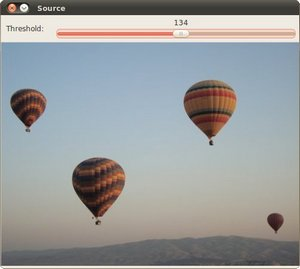
\includegraphics[width=0.8\linewidth]{test}
% %\end{figure}
% \end{frame}

% %------------------------------------------------

% \begin{frame}[fragile] % Need to use the fragile option when verbatim is used in the slide
% \frametitle{Citation}
% An example of the \verb|\cite| command to cite within the presentation:\\~

% This statement requires citation \cite{p1}.
% \end{frame}

% %------------------------------------------------

% \begin{frame}
% \frametitle{References}
% \footnotesize{
% \begin{thebibliography}{99} % Beamer does not support BibTeX so references must be inserted manually as below
% \bibitem[Smith, 2012]{p1} John Smith (2012)
% \newblock Title of the publication
% \newblock \emph{Journal Name} 12(3), 45 -- 678.
% \end{thebibliography}
% }
% \end{frame}

%------------------------------------------------
\section{Closing Remarks}
	\begin{frame}
	\Huge{\centerline{The End}}
	\end{frame}

%----------------------------------------------------------------------------------------

\end{document} 